%!TEX root = ../../../tugas-akhir.tex
\section{Implementasi Algoritma Paralel pada Library big integer}
  \subsection{Lingkungan Implementasi} \label{sec:impl_env}
    Sesuai dengan pertimbangan pada subbab \ref{sec:parallel_env}, implementasi algoritma paralel akan dilakukan dengan menggunakan pthread. Implementasi akan dilakukan menggunakan \textit{compiler} GCC versi 5.4.0 dan dijalankan pada sistem operasi Ubuntu 18.04 64-bit. Penggunaan TLS akan diuji pada penggunaan HTTPS pada web server yang diinstall pada sistem operasi. Web server yang digunakan adalah Apache2 dengan menggunakan modul tambahan mod\_ssl. Arsitektur sistem yang digunakan dapat dilihat pada Gambar \ref{fig:openssl_arch}

    \begin{figure}[h]
      \centering
      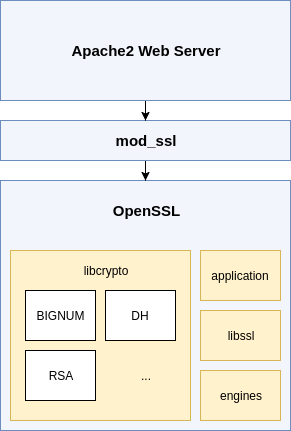
\includegraphics[width=0.4\textwidth]{resources/img/ch-4/implementation_arch.png}
      \caption{Arsitektur OpenSSL}
      \label{fig:openssl_arch}
    \end{figure}

    % Cek lagi jumlahnya
    Secara default, jumlah maksimal thread maksimum yang akan digunakan oleh OpenSSL untuk menjalankan komputasi big integer secara paralel akan bergantung pada jumlah core yang terdapat pada lingkungan instalasi. Dalam aplikasi yang membutuhkan komputasi yang tinggi setiap thread akan berjalan secara terus menerus. Dengan demikian jumlah thread maksimum akan sama dengan jumlah aplikasi. Namun, aplikasi juga memiliki pilihan konfigurasi untuk menentukan jumlah thread maksimum yang dapat digunakan.
    % \todo{cite disini}

  \subsection{Batasan Implementasi}
    Implementasi dilakukan pada sistem operasi Ubuntu 64 bit. Karena itu, implementasi library big number hanya berfokus pada openssl dengan yang memiliki konfigurasi makro sebagai berikut:

    \begin{enumerate}[label=\roman*.]
      \item BN\_ULONG = unsigned long
      \item OPENSSL\_SMALL\_FOOTPRINT = false
      \item BN\_MUL\_COMBA = true
      \item BN\_RECURSION = true
      \item BN\_CTX\_POOL\_SIZE = 16
    \end{enumerate}
    % \todo{masukin lampiran?}
    Konfigurasi makro tersebut digunakan dalam pemilihan dan manajemen struktur data yang digunakan serta pemilihan algoritma pada bagian tertentu. Sebagai contoh, algoritma yang digunakan dalam perkalian adalah algoritma karatsuba dan algoritma comba pada basis rekursif.


  \subsection{Struktur File \textit{Source Code}}

    \begin{figure}[h]
      \centering
      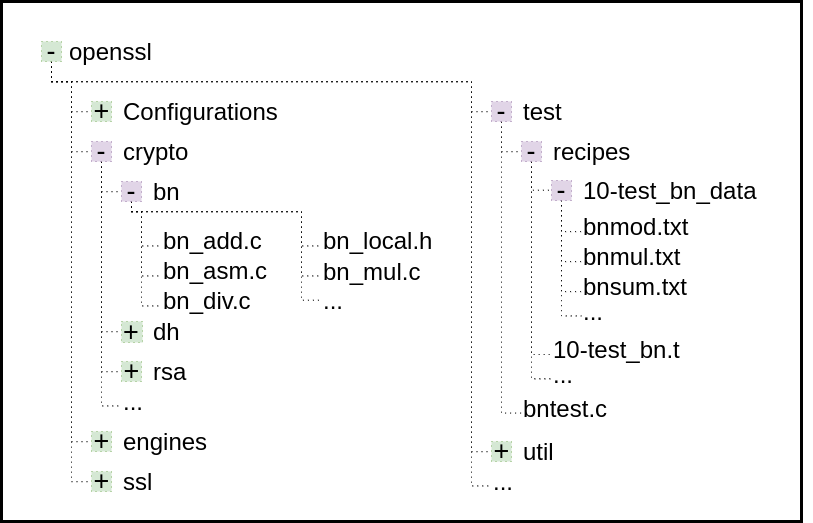
\includegraphics[width=0.8\textwidth]{resources/img/ch-4/file-tree.png}
      \caption{Struktur Source Code OpenSSL}
      \label{fig:ossl_file_structure}
    \end{figure}

    Struktur \textit{source code} dapat dilihat pada Gambar \ref{fig:ossl_file_structure}. Direktori utama berisi pembagian dari fungsi aplikasi yang ada dalam OpenSSL. Beberapa fungsi tersebut adalah direktori |doc| yang berisi dokumentasi OpenSSL, |crypto| yang berisi library kriptografi, |ssl| yang berisi dari library komunikasi ssl, serta |test| yang berisi unit test yang dimiliki OpenSSL.

    Direktori |crypto| berisi modul-modul yang membentuk libcrypto, dengan setiap modul terbentuk dalam sebuah direktori yang berbeda. Modul |bn| merupakan modul yang mengatasi perhitungan operasi aritmatika big integer. Selain itu, modul |dh| dan |rsa| merupakan modul yang menangani komputasi Diffie-Hellman dan RSA pada OpenSSL.

    Modul |bn| memiliki beberapa submodul masing-masing merupakan file yang berbeda. Setiap submodul sendiri mengatasi fungsi yang terkait dengan submodul tersebut, ataupun operasi yang komputasinya mirip dengan submodul. Sebagai contoh, submodul |bn_add| merupakan submodul yang mengatasi operasi penjumlahan dan pengurangan pada big integer. Selain itu, submodul |bn_mul| merupakan submodul yang mengatasi operasi perkalian serta pemilihan algoritma perkalian yang digunakan dalam OpenSSL.

    Direktori |test| dan |util| merupakan direktori yang digunakan dalam \textit{unit test} OpenSSL. Dalam direktori ini terdapat kasus uji dan script yang digunakan dalam unit test untuk setiap modul untuk melakukan test terhadap fungsionalitas OpenSSL. Penjelasan lebih jauh terhadap pengujian fungsionalitas OpenSSL dapat dilihat pada subbab \ref{sec:func_testing}

  \subsection{Struktur Data Big Integer} \label{sec:bignum_struct}
  \subsubsection{Struktur BIGNUM}

    Pada OpenSSL, sebuah big integer direpresentasikan dalam struktur data |BIGNUM|. |BIGNUM| terdiri dari sebuah array dengan ukuran dinamis dan beberapa variabel integer yang menyimpan informasi tambahan. Dengan demikian secara teori |BIGNUM| tidak memiliki nilai maksimum. Untuk keperluan paralelisasi, |BIGNUM| dapat digunakan tanpa mengubah strukturnya sedikitpun. BIGNUM sendiri merupakan sebuah \textit{struct} yang memiliki deklarasi sesuai pada Source Code \ref{code:bignum_st}.

    \begin{lstlisting}[caption={Struktur Data bignum}, label={code:bignum_st}]
struct bignum_st {
       BN_ULONG *d;
       int top;
       int dmax;
       int neg;
       int flags;
};
    \end{lstlisting}

    |BN_ULONG| sendiri adalah sebuah makro yang menggantikan |unsigned long|.

    |d| adalah pointer untuk array of integer.

    |top| merupakan index |d| yang terakhir digunakan plus satu.

    |dmax| adalah panjang maksimum array yang telah dibuat. |neg| bernilai satu jika BIGNUM bernilai negatif.

    \subsubsection{Struktur BN\_CTX}

    Setiap kali pembuatan struktur data |BIGNUM| terjadi alokasi memori yang memiliki overhead yang cukup tinggi jika dilakukan berulang ulang \citep{doc_bnctx}. Sementara itu, operasi aritmatika kompleks seperti perkalian dengan algoritma karatsuba, pembagian, atau perpangkatan modulo membutuhkan beberapa struktur |BIGNUM| yang digunakan untuk menyimpan variabel sementara. Struktur data |BN_CTX| menyimpan sejumlah variabel |BIGNUM| yang dapat digunakan dalam operasi aritmatika, dengan demikian program tidak pelu melakukan alokasi memori setiap kali program membutuhkan sebuah struktur |BIGNUM|.

    % jelasin lebih jauh

    \begin{lstlisting}[caption={Struktur bignum\_ctx}, label={code:bignum_ctx}]
struct bignum_ctx {
    BN_POOL pool;
    BN_STACK stack;
    unsigned int used;
    int err_stack;
    int too_many;
    int flags;
};

/* BN_POOL */
typedef struct bignum_pool_item {
    BIGNUM vals[BN_CTX_POOL_SIZE];
    struct bignum_pool_item *prev, *next;
} BN_POOL_ITEM;
typedef struct bignum_pool {
    BN_POOL_ITEM *head, *current, *tail;
    unsigned used, size;
} BN_POOL;

/* BN_STACK */
typedef struct bignum_ctx_stack {
    unsigned int *indexes;
    unsigned int depth, size;
} BN_STACK;
    \end{lstlisting}

    Struktur dari |BN_CTX| dapat dilihat pada Source Code \ref{code:bignum_ctx}. |BN_CTX| terdiri dari kumpulan |BIGNUM| yang disimpan pada |BN_POOL| serta |BN_STACK| yang menyimpan jumlah |BIGNUM| yang digunakan oleh sebuah fungsi. |BN_POOL| merupakan list of array dengan panjang array sebesar |BN_CTX_POOL_SIZE|. |BN_STACK| digunakan untuk menyimpan jumlah BIGNUM yang digunakan dalam sebuah fungsi.

    Fungsi yang menggunakan |BN_CTX| harus memanggil |BN_CTX_start()| sebelum penggunaan |BN_CTX| dan memanggil |BN_CTX_end()| setelah pemanggilan |BN_CTX|. Dua fungsi tersebut akan menyimpan dan menghitung jumlah BIGNUM yang didapat dari pemanggilan |BN_CTX_get()| pada fungsi tersebut.

    \subsubsection{Struktur Data untuk Paralelisasi}
    Terdapat beberapa struktur data tambahan yang dibuat untuk paralelisasi fungsi menggunakan pthread. Pemanggilan fungsi oleh pthread membutuhkan sebuah fungsi yang menerima satu argumen dengan tipe |void *|. Agar fungsi yang dijalankan secara paralel dapat mengolah lebih dari satu data, dibuat \textit{struct} khusus untuk setiap fungsi tersebut. Struktur data yang dibuat untuk digunakan oleh fungsi paralel dapat dilihat pada \textit{Source Code} \ref{code:parallel_struct}.

    \begin{lstlisting}[caption={Struktur Data Paralelisasi}, label={code:parallel_struct}]
typedef struct _add_sub_args_st {
    BN_ULONG *r;
    const BN_ULONG *a;
    const BN_ULONG *b;
    int n;
    int id;
    char type;
    BN_ULONG carry;
} add_sub_args;

typedef struct _mul_normal_args_st {
    BN_ULONG *r;
    const BN_ULONG *a;
    BN_ULONG w;
    int n;
    BN_ULONG carry;
} mul_normal_args;

typedef struct _recursive_args_st {
    BN_ULONG *r;
    BN_ULONG *a;
    BN_ULONG *b;
    int n2;
    int dna;
    int dnb;
    BN_ULONG *t;
    int *used_thr;
} recursive_args;
    \end{lstlisting}

  \subsection{Implementasi Modul Operasi Aritmatika}

    \subsubsection{Submodul Penjumlahan dan Pengurangan}
  Submodul penjumlahan dan pengurangan terdapat pada file |bn/BN_add.c|. Fungsi |BN_add()| pada adalah melakukan pengolahan data pada a dan b seperti mengecek negatif dan mengecek panjang masing-masing array. Jika a dan b memiliki tanda yang berbeda, akan dipanggil fungsi |BN_usub()| selain itu akan dipanggil fungsi |BN_uadd()|.

  |BN_uadd()| dan |BN_usub()| melakukan pengolahan data pada a dan b sehingga terdapat dua representasi array yang dapat diolah oleh |BN_add_words()| dan |BN_sub_words()|. Daftar fungsi yang terdapat pada submodul penjumlahan dan pengurangan dapat dilihat pada Tabel \ref{tab:bn_add_func}.

  \begin{table}[!h]
    \caption{Fungsi dalam submodul penjumlahan dan pengurangan}
    \label{tab:bn_add_func}
    \begin{tabular}{R{2.8cm}L{10.5cm}}
      \toprule
      \textbf{Header Fungsi} & |int BN_add(BIGNUM *r, const BIGNUM *a, const BIGNUM *b)|    \\ \midrule
      \textit{Deskripsi}     & Menjumlahkan a dan b dan menyimpan hasilnya pada r $(a+b=r)$ \\
      \textit{Prekondisi}    & -                                                            \\
      \textit{Return Value}  & 1 jika fungsi berhasil dilakukan dan 0 jika tidak
      \\ \bottomrule
      \textbf{Header Fungsi} & |int BN_sub(BIGNUM *r, const BIGNUM *a, const BIGNUM *b)|    \\ \midrule
      \textit{Deskripsi}     & Mengurangi b dari a dan menyimpan hasilnya pada r $(a-b=r)$  \\
      \textit{Prekondisi}    & -                                                            \\
      \textit{Return Value}  & 1 jika fungsi berhasil dilakukan dan 0 jika tidak
      \\ \bottomrule
      \textbf{Header Fungsi} & |int BN_uadd(BIGNUM *r, const BIGNUM *a, const BIGNUM *b)|   \\ \midrule
      \textit{Deskripsi}     & Menjumlahkan a dan b dan menyimpan hasilnya pada r $(a+b=r)$ \\
      \textit{Prekondisi}    & $a \geq 0$, $ b \geq 0$                                      \\
      \textit{Return Value}  & 1 jika fungsi berhasil dilakukan dan 0 jika tidak
      \\ \bottomrule
      \textbf{Header Fungsi} & |int BN_usub(BIGNUM *r, const BIGNUM *a, const BIGNUM *b)|   \\ \midrule
      \textit{Deskripsi}     & Mengurangi b dari a dan menyimpan hasilnya pada r $(a-b=r)$  \\
      \textit{Prekondisi}    & $a \geq 0$, $b \geq 0$, $a \geq b$                           \\
      \textit{Return Value}  & 1 jika fungsi berhasil dilakukan dan 0 jika tidak
      \\ \bottomrule
    \end{tabular}
  \end{table}

  |BN_add_words()| dan |BN_sub_words()| bukan merupakan bagian dari submodul ini, namun dalam submodul asm. Submodul asm dijelaskan lebih lanjut pada subbab \ref{sec:bn_asm}. Dua fungsi tersebut menerima masukan dua array dengan ukuran yang sama dan menjumlahkannya secara sekuensial. Penerapan algoritma paralel \ref{alg:add} pada OpenSSL terdapat pada fungsi ini.

    \subsubsection{Submodul Perkalian}
  Submodul perkalian terdapat pada file |bn/bn_mul.c|. Fungsi |bn_mul()| merupakan fungsi yang akan dipanggil untuk melakukan operasi perkalian big integer. Terdapat dua algoritma perkalian yang diimplementasikan dalam modul ini, yaitu algoritma perkalian panjang pada |bn_mul_normal()| dan algoritma perkalian karatsuba pada |bn_mul_recursive()|. Daftar fungsi yang relevan pada submodul ini dapat dilihat pada Tabel \ref{tab:bn_mul}.

  \begin{table}[h]
    \caption{Fungsi dalam submodul perkalian}
    \label{tab:bn_mul}
    \begin{tabular}{R{2.8cm}L{10.5cm}}

      \toprule
      \textbf{Header Fungsi} & |int BN_mul(BIGNUM *r, const BIGNUM *a, const BIGNUM *b, BN_CTX *ctx)| \\ \midrule
      \textit{Deskripsi}     & Mengalikan $b$ pada $a$ dan menyimpan hasilya dalam $r, (r = a * b)$.\\
      \textit{Prekondisi}    & -\\
      \textit{Return Value}  & 1 jika fungsi berhasil dilakukan dan 0 jika tidak
      \\ \bottomrule

      \textbf{Header Fungsi} & |void bn_mul_normal(BN_ULONG *r, BN_ULONG *a, int na, BN_ULONG *b, int nb)| \\ \midrule
      \textit{Deskripsi}     & Perkalian $a$ dan $b$ dengan menggunakan algoritma perkalian panjang, $a$ dan $b$ adalah array yang merepresentasikan operand perkalian.  \\
      \textit{Prekondisi}    & $na = length(a)$, $nb = length(b)$ \\
      \textit{Return Value}  & 1 jika fungsi berhasil dilakukan dan 0 jika tidak
      \\ \bottomrule

      \textbf{Header Fungsi} & |void bn_mul_recursive(BN_ULONG *r, BN_ULONG *a, BN_ULONG *b, int n2 int dna, int dnb, BN_ULONG *t)| \\ \midrule
      \textit{Deskripsi}     & Perkalian $a$ dan $b$ dengan menggunakan algoritma perkalian karatsuba. $n2$ adalah panjang hasil perkalian \\
      \textit{Prekondisi}    & $length(r) = 2*n2$. $ length(t) = 2*n2$. $n2 = 2^k, k \in \mathbb{Z} $. $dna = length(a) - n2$. $dnb = length(b) - n2$ \\
      \textit{Return Value}  & 1 jika fungsi berhasil dilakukan dan 0 jika tidak
      \\ \bottomrule
    \end{tabular}
  \end{table}

  Algoritma perkalian comba hanya digunakan untuk |BIGNUM| yang memiliki panjang 4 atau 8 word. Implementasi ini dilakukan karena untuk jumlah word yang lebih tinggi, perkalian comba tidak menghasilkan hasil yang lebih baik dibandingkan dengan perkalian biasa. Implementasi algoritma perkalian comba terdapat pada fungsi |bn_mul_comba4()| dan |bn_mul_comba8()| di submodul asm.

  Basis yang dipilih dalam perkalian karatsuba adalah ketika dua operand memiliki panjang 8 word. Ketika perkalian karatsuba mencapai basis, akan dipanggil algoritma perkalian comba dalam fungsi |bn_mul_comba8()|. Implementasi algoritma paralel karatsuba dalam pseudocode \ref{alg:parallel_karatsuba} diimplementasikan pada fungsi |bn_mul_recursive()| ini.

  Algoritma perkalian panjang pada fungsi |bn_mul_normal()| akan memanggil fungsi |bn_mul_add_words()| dari submodul asm. Fungsi |bn_mul_add_words| inilah tempat algoritma paralel \ref{alg:mul_parallel} diimplementasikan.
  % \todo{tambahin ref}

  \begin{lstlisting}[caption={Struktur Data recursive\_args}, label={code:par_st}]
typedef struct _recursive_args_st {
    BN_ULONG *r;
    BN_ULONG *a;
    BN_ULONG *b;
    int n2;
    int dna;
    int dnb;
    BN_ULONG *t;
    int used_thr;
} recursive_args;
  \end{lstlisting}

  Terdapat strukur data tambahan yang dibuat pada submodul ini agar pemanggilan fungsi secara rekursif dapat dilakukan oleh pthread. Struct |recursive_args| berisi argumen yang dibutuhkan oleh |bn_mul_recursive()| serta \textit{counter} jumlah thread yang sudah dijalankan. \textit{Counter} jumlah thread digunakan untuk membatasi thread yang dipanggil agar tidak melebihi jumlah thread maksimum. Pemanggilan jumlah thread yang lebih besar dari jumlah thread maksimum mungkin menyebabkan \textit{false sharing} yang akan menurunkan kinerja submodul ini.

    \subsubsection{Submodul Pembagian}
  Submodul pembagian terdapat pada file |bn/bn_div.c|. Fungsi |BN_div()| merupakan implementasi algoritma pembagian panjang pada OpenSSL. Sesuai dengan penjelasan pada subbab \ref{sec:div_theory}, algoritma pembagian panjang membutuhkan divisor yang telah ternormalisasi. Proses normalisasi pada implementasi ini dilakukan dengan melakukan \textit{left shift} pada divisor sehingga bit paling signifikan yang dimiliki divisor bernilai 1. Proses normalisasi divisor dilakukan oleh fungsi |bn_left_align()|, sementara itu proses \textit{left shift} pada bilangan dibagi dilakukan oleh |bn_lshift_fixed_top()| yang terdapat pada submodul |bn_shift|.
  % \todo[inline]{cek lagi istilahnya, sesuaikan sama bab 2 (divisor, number, quotient, remainder)}

  \begin{table}[h]
    \caption{Fungsi dalam submodul pembagian}
    \begin{tabular}{R{2.8cm}L{10.5cm}}
      \toprule
      \textbf{Header Fungsi} & |BN_div(BIGNUM *dv, BIGNUM *rm, const BIGNUM *num, const BIGNUM *divisor, BN_CTX *ctx)|                                                                                                       \\ \midrule
      \textit{Deskripsi}     & Membagi num dengan divisor, hasil pembagian disimpan sebagai dv dan sisa pembagian disimpan sebagai rm. Baik div maupun rm bisa menjadi NULL jika hasil atau sisa pembagian tidak dibutuhkan. \\
      \textit{Prekondisi}    & - \\
      \textit{Return Value}  & 1 jika fungsi berhasil dilakukan dan 0 jika tidak
      \\ \bottomrule
      \textbf{Header Fungsi} & |int bn_left_align(BIGNUM *num)|                                                                                                                                                              \\ \midrule
      \textit{Deskripsi}     & Normalisasi divisor BIGNUM $num$ agar $num > \beta/2$  \\
      \textit{Prekondisi}    & - \\
      \textit{Return Value}  & 1 jika fungsi berhasil dilakukan dan 0 jika tidak
      \\ \bottomrule
    \end{tabular}
  \end{table}

    \subsubsection{Submodul Asm} \label{sec:bn_asm}
  Submodul asm terdapat pada file |bn/bn_asm.c|. Submodul ini terdiri dari fungsi yang melakukan operasi langsung terhadap array yang ada didalam struktur BIGNUM. Sebagai contoh, |bn_add_words()| merupakan fungsi yang menjumlahkan dua array dengan ukuran yang sama dan menyimpannya pada sebuah array yang baru. Sebagian besar fungsi yang terdapat dalam submodul ini merupakan fungsi yang dapat diimplementasikan dalam assembly dengan sederhana sehingga kinerja yang dihasilkan lebih baik.

  Beberapa implementasi Pseudocode dari subbab \ref{sec:parallelization} diimplementasikan pada submodul ini. Implementasi dilakukan pada submodul ini karena submodul ini merupakan modifikasi big integer pada level terrendah dalam modul BIGNUM. Dengan demikian, implementasi pada submodul ini akan digunakan oleh submodul-submodul lain dalam modul bignum yang menggunakan fungsi low level.

  Terdapat satu struktur data tambahan yang dibuat dalam submodul ini. Struktur data dibuat karena penggunaan pthread terhadap fungsi hanya dapat menerima satu argumen dengan tipe data |void*|. Agar thread dapat mengolah data lebih dari satu, perlu dibuat sebuah struct yang berisi argumen dari fungsi awal. Akan dilakukan type casting antara struct yang dibuat dan |void*| dalam setiap pemanggilan thread. Strukur data yang dibuat dalam submodul ini dapat dilihat pada Source Code \ref{code:par_st}. Struktur data yang digunakan untuk penjumlahan adalah |add_args|

  \begin{table}[h]
    \caption{Fungsi dalam submodul asm}
    \begin{tabular}{R{2.8cm}L{10.5cm}}
      \toprule
      \textbf{Header Fungsi} & |BN_ULONG bn_add_words(BN_ULONG *r, const BN_ULONG *a, const BN_ULONG *b, int n)|  \\ \midrule
      \textit{Deskripsi} & Menjumlahkan dua array a dan b ($a+b$) yang merupakan variabel |d| dari |BIGNUM| dan menyimpan hasilnya pada array r.                                                                                     \\
      \textit{Prekondisi}    & $length(a) = length(b) = n$                                 \\
      \textit{Return Value}  & Carry
      \\ \bottomrule
      \textbf{Header Fungsi} & |BN_ULONG bn_sub_words(BN_ULONG *r, const BN_ULONG *a, const BN_ULONG *b, int n)|  \\ \midrule
      \textit{Deskripsi} & Mengurangi dua array b dari array a ($a-b$) yang merupakan variabel |d| dari |BIGNUM| dan menyimpan hasilnya pada array r.                                                                                     \\
      \textit{Prekondisi}    & $length(a) = length(b) = length(r) n$                                 \\
      \textit{Return Value}  & Carry
      \\ \bottomrule
      \textbf{Header Fungsi} & |BN_ULONG bn_mul_words(BN_ULONG *rp, const BN_ULONG *ap, int num, BN_ULONG w)|     \\ \midrule
      \textit{Deskripsi} & Mengalikan array ap terhadap sebuah elemen w dan menyimpan hasilnya pada rp. ($rp = ap * w$)                                                                                      \\
      \textit{Prekondisi}    & $length(ap) = length(rp) = num$ -                                                                                  \\
      \textit{Return Value}  & Carry
      \\ \bottomrule
      \textbf{Header Fungsi} & |BN_ULONG bn_mul_add_words(BN_ULONG *rp, const BN_ULONG *ap, int num, BN_ULONG w)| \\ \midrule
      \textit{Deskripsi} & Mengalikan array ap terhadap w, menjumlahkan hasilnya dengan a, dan menyimpannya pada rp. ($rp = ap + ap * w$)                                                                                    \\
      \textit{Prekondisi}    & $length(ap) = length(rp) = num$ -                                                                                  \\
      \textit{Return Value}  & Carry
      \\ \bottomrule
      \textbf{Header Fungsi} & |BN_ULONG bn_div_words(BN_ULONG h, BN_ULONG l, BN_ULONG d)|                        \\ \midrule
      \textit{Deskripsi}  & Membagi bilangan dua word $hl$ dengan bilangan satu word $d$ dan mengembalikan hasilnya.                                                                                   \\
      \textit{Prekondisi}    & - -                                                                                  \\
      \textit{Return Value}  & Hasil pembagian
      \\ \bottomrule
      \textbf{Header Fungsi} & |void bn_mul_comba8(BN_ULONG *r, BN_ULONG *a, BN_ULONG *b)|                        \\ \midrule
      \textit{Deskripsi} &  Mengalikan bilangan 8 word a dan b dan menyimpan hasilnya pada r. ($r = a*b$)                                                                                    \\
      \textit{Prekondisi}    & $length(a) = length(b) = 8, length(r) = 16$ -                                                                                  \\
      \textit{Return Value}  & -
      \\ \bottomrule
    \end{tabular}
  \end{table}

